\documentclass[a4paper,12pt]{article}
\usepackage[utf8]{inputenc}
\usepackage[russian]{babel}
\usepackage{amsmath}
\usepackage{amssymb}
\usepackage{enumitem}
\usepackage{graphicx}
\usepackage{hyperref}
\usepackage[a4paper, top= 1cm, bottom=2cm, left=2cm, right=2cm]{geometry}

\hypersetup{
    colorlinks=true,
    linkcolor=blue,
    urlcolor=blue, 
}

\title{Оценка + пример 2.0}

\begin{document}
\maketitle
    \subsection*{Задачи}
    \begin{enumerate}
        \item Натуральные числа от 1 до 10 разбили на две группы так, что произведение чисел в первой группе делится на произведение чисел во второй группе. Какое наименьшее значение может принимать частное от деления первого произведения на второе?
        \item Каково наименьшее натуральное $n$ такое, что $n!$ делится на 18, на 19, на 20 и на 21?  
        \item \begin{enumerate}
            \item Какое наименьшее число выстрелов в игре "Морской бой" на доске $8 \cdot 8$ нужно сделать, чтобы наверняка ранить четырехпалубный корабль (четырехпалубный корабль состоит из четырех клеток, расположенных в один ряд)?
            \item А на доске $7 \cdot 7$?
        \end{enumerate}
        \item Фальшивомонетчик Вася изготовил четыре монеты достоинством 1, 3, 4, 7 квача, которые должны весить 1, 3, 4, 7 граммов соответственно. Но одну из этих монет он сделал некачественно – с неправильным весом. За какое наименьшее количество взвешиваний на чашечных весах без гирь можно гарантированно определить неправильную монету?
        \item Среди пяти внешне одинаковых монет 3 настоящие и две фальшивые, одинаковые по весу, но неизвестно, тяжелее или легче настоящих. Как за наименьшее число взвешиваний найти хотя бы одну настоящую монету?
        \item В пруд пустили 30 щук, которые постепенно поедают друг друга. Щука считается сытой, если она съела не менее трёх щук (сытых или голодных). Какое наибольшее число щук может насытиться?
    \end{enumerate}
    \subsection*{Примеры и контрпримеры}
    \begin{enumerate}
        \item Гриб называется плохим, если в нём не менее 10 червей. В лукошке 90 плохих и 10 хороших грибов. Могут ли все грибы стать хорошими после того, как некоторые черви переползут из плохих грибов в хорошие?
        \item Использовав каждую из цифр от 0 до 9 ровно по разу, запишите 5 ненулевых чисел так, чтобы каждое делилось на предыдущее.
        \item Нарисуйте фигуру, которую можно разрезать на четыре фигурки, изображённые слева, а можно – на пять фигурок, изображенных справа, учитывая, что их можно поворачивать.
        \begin{figure}[h]
            \centering
            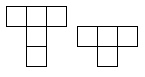
\includegraphics[width=0.15\linewidth]{image.png}
        \end{figure}
    \end{enumerate}
\end{document}
